\documentclass{article}

\usepackage{tikz}
\usetikzlibrary{arrows}

\usepackage[font={small,sf},labelfont={bf},labelsep=endash]{caption}
\usepackage{relsize}
\usepackage{xspace}

\newcommand{\hisparc}{\textsmaller{HiSPARC}\xspace}
\newcommand{\labview}{\textsmaller{LabVIEW}\xspace}


% Defines a `datastore' shape for use in DFDs.  This inherits from a
% rectangle and only draws two horizontal lines.

\makeatletter
\pgfdeclareshape{datastore}{
  \inheritsavedanchors[from=rectangle]
  \inheritanchorborder[from=rectangle]
  \inheritanchor[from=rectangle]{center}
  \inheritanchor[from=rectangle]{base}
  \inheritanchor[from=rectangle]{north}
  \inheritanchor[from=rectangle]{north east}
  \inheritanchor[from=rectangle]{east}
  \inheritanchor[from=rectangle]{south east}
  \inheritanchor[from=rectangle]{south}
  \inheritanchor[from=rectangle]{south west}
  \inheritanchor[from=rectangle]{west}
  \inheritanchor[from=rectangle]{north west}
  \backgroundpath{
    %  store lower right in xa/ya and upper right in xb/yb
    \southwest \pgf@xa=\pgf@x \pgf@ya=\pgf@y
    \northeast \pgf@xb=\pgf@x \pgf@yb=\pgf@y
    \pgfpathmoveto{\pgfpoint{\pgf@xa}{\pgf@ya}}
    \pgfpathlineto{\pgfpoint{\pgf@xb}{\pgf@ya}}
    \pgfpathmoveto{\pgfpoint{\pgf@xa}{\pgf@yb}}
    \pgfpathlineto{\pgfpoint{\pgf@xb}{\pgf@yb}}
 }
}
\makeatother


\begin{document}

\begin{figure}
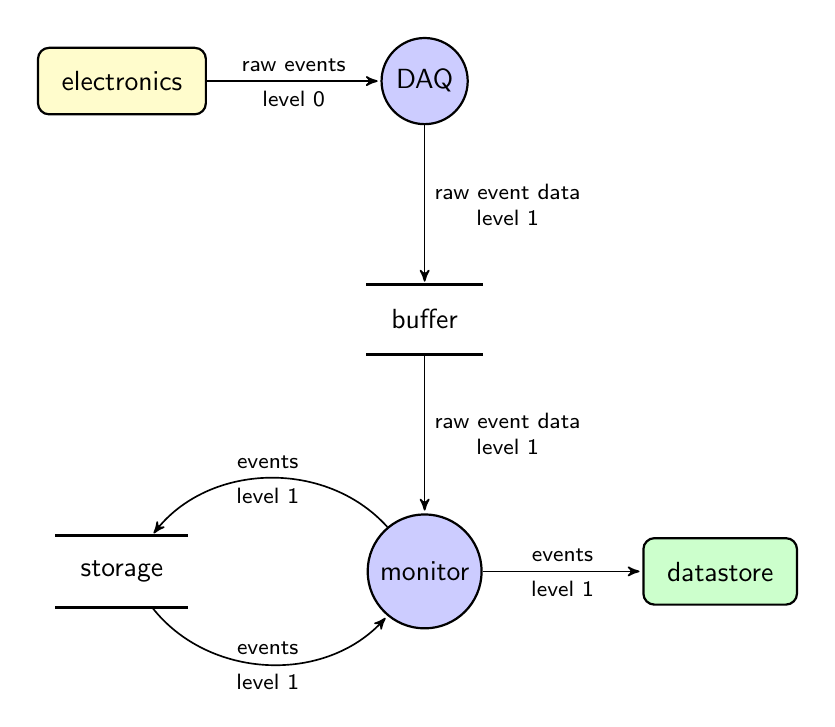
\begin{tikzpicture}
[font=\sffamily,
 every matrix/.style={ampersand replacement=\&,column sep=2cm,row sep=2cm},
 source/.style={draw,thick,rounded corners,fill=yellow!20,inner sep=.3cm},
 process/.style={draw,thick,circle,fill=blue!20},
 sink/.style={source,fill=green!20},
 datastore/.style={draw,very thick,shape=datastore,inner sep=.3cm},
 dots/.style={gray,scale=2},
 to/.style={->,>=stealth',shorten >=1pt,semithick,font=\sffamily\footnotesize},
 every node/.style={align=center},
]

% Position the nodes using a matrix layout
\matrix{
  \node[source] (hisparcbox) {electronics};
    \& \node[process] (daq) {DAQ}; \& \\

  \& \node[datastore] (buffer) {buffer}; \& \\

  \node[datastore] (storage) {storage};
    \& \node[process] (monitor) {monitor};
    \& \node[sink] (datastore) {datastore}; \\
};

% Draw the arrows between the nodes and label them.
\draw[to] (hisparcbox) -- node[midway,above] {raw events}
    node[midway,below] {level 0} (daq);
\draw[to] (daq) -- node[midway,right] {raw event data\\level 1} (buffer);
\draw[to] (buffer) --
    node[midway,right] {raw event data\\level 1} (monitor);
\draw[to] (monitor) to[bend right=50] node[midway,above] {events}
    node[midway,below] {level 1} (storage);
\draw[to] (storage) to[bend right=50] node[midway,above] {events}
    node[midway,below] {level 1} (monitor);
\draw[to] (monitor) -- node[midway,above] {events}
    node[midway,below] {level 1} (datastore);
\end{tikzpicture}

\caption{Data flow diagram of a \hisparc station PC.  A \labview program
communicates with the \hisparc II electronics.  Data is sanitized and,
along with preliminary analysis results and configuration settings, sent
to the \emph{buffer}.  The monitor program retrieves raw event data from
the buffer and creates structured array data.  The events are then stored
in the \emph{storage}.  When a batch of events is ready, it is retrieved
from the storage and uploaded over the internet to the datastore.}
\end{figure}

\end{document}
